%\title{Modelo de Projeto de pesquisa}
%% abtex2-modelo-projeto-pesquisa.tex, v-1.9 laurocesar
%% Copyright 2012-2013 by abnTeX2 group at http://abntex2.googlecode.com/ 
%%
%% This work may be distributed and/or modified under the
%% conditions of the LaTeX Project Public License, either version 1.3
%% of this license or (at your option) any later version.
%% The latest version of this license is in
%%   http://www.latex-project.org/lppl.txt
%% and version 1.3 or later is part of all distributions of LaTeX
%% version 2005/12/01 or later.
%%
%% This work has the LPPL maintenance status `maintained'.
%% 
%% The Current Maintainer of this work is the abnTeX2 team, led
%% by Lauro César Araujo. Further information are available on 
%% http://abntex2.googlecode.com/
%%
%% This work consists of the files abntex2-modelo-projeto-pesquisa.tex
%% and abntex2-modelo-references.bib
%%

% ------------------------------------------------------------------------
% ------------------------------------------------------------------------
% abnTeX2: Modelo de Projeto de pesquisa em conformidade com 
% ABNT NBR 15287:2011 Informação e documentação - Projeto de pesquisa -
% Apresentação 
% ------------------------------------------------------------------------ 
% ------------------------------------------------------------------------

\documentclass[
    % -- opções da classe memoir --
    12pt,               % tamanho da fonte
    %openright,          % capítulos começam em pág ímpar (insere página vazia caso preciso)
    oneside,%twoside,            % para impressão em verso e anverso. Oposto a oneside
    a4paper,            % tamanho do papel. 
    % -- opções da classe abntex2 --
    %chapter=TITLE,     % títulos de capítulos convertidos em letras maiúsculas
    %section=TITLE,     % títulos de seções convertidos em letras maiúsculas
    %subsection=TITLE,  % títulos de subseções convertidos em letras maiúsculas
    %subsubsection=TITLE,% títulos de subsubseções convertidos em letras maiúsculas
    % -- opções do pacote babel --
    english,            % idioma adicional para hifenização
    french,             % idioma adicional para hifenização
    spanish,            % idioma adicional para hifenização
    brazil,             % o último idioma é o principal do documento
    ]{abntex2}



% ---
% PACOTES
% ---

% ---
% Pacotes fundamentais 
% ---
\usepackage{lmodern}            % Usa a fonte Latin Modern
\usepackage[T1]{fontenc}        % Selecao de codigos de fonte.
\usepackage[utf8]{inputenc}     % Codificacao do documento (conversão automática dos acentos)
\usepackage{indentfirst}        % Indenta o primeiro parágrafo de cada seção.
\usepackage{color}              % Controle das cores
\usepackage{graphicx}           % Inclusão de gráficos
\usepackage{microtype}          % para melhorias de justificação
%\usepackage[utf8x]{inputenc} 
% ---


% ---
% Pacotes adicionais, usados apenas no âmbito do Modelo Canônico do abnteX2
% ---
\usepackage{lipsum}             % para geração de dummy text
% ---

% ---
% Pacotes de citações
% ---
%\usepackage[brazilian,hyperpageref]{backref} % Paginas com as citações na bibl
%\usepackage[alf]{abntex2cite}   % Citações padrão ABNT

% --- 
% CONFIGURAÇÕES DE PACOTES
% --- 

% ---
% Configurações do pacote backref
% Usado sem a opção hyperpageref de backref
%\renewcommand{\backrefpagesname}{Citado na(s) página(s):~}
% Texto padrão antes do número das páginas
%\renewcommand{\backref}{}
% Define os textos da citação
%\renewcommand*{\backrefalt}[4]{
%    \ifcase #1 %
 %       Nenhuma citação no texto.%
  %  \or
   %     Citado na página #2.%
   % \else
   %     Citado #1 vezes nas páginas #2.%
   % \fi}%
% ---

% ---
% Informações de dados para CAPA e FOLHA DE ROSTO
% ---
\titulo{Desenvolvimento de algoritmos genéticos em sistemas de hardware reconfigurável}
\autor{José Randson da Cunha}
\local{Natal}
\data{Junho,2016}
\instituicao{%

  \par
  Orientador
  \par
  \textbf{Prof. Dr. Marcelo Augusto Costa Fernandes}

  Universidade Federal do Rio Grande do Norte - UFRN
  \par
  Departamento de engenharia de computação e automação
  }
\tipotrabalho{Trabalho de conlusão de curso (Graduação)}
% O preambulo deve conter o tipo do trabalho, o objetivo, 
% o nome da instituição e a área de concentração 
\preambulo{Trabalho de conclusão de curso de
          Graduação apresentado ao
          Departamento de Engenharia de
          Computação e Automação do Centro
          de Tecnologia da Universidade
          Federal do Rio Grande do Norte como
          requisito para a obtenção do título de
          Engenheiro de Computação.}
% ---

% ---
% Configurações de aparência do PDF final

% alterando o aspecto da cor azul
\definecolor{blue}{RGB}{41,5,195}

% informações do PDF
\makeatletter
\hypersetup{
        %pagebackref=true,
        pdftitle={\@title}, 
        pdfauthor={\@author},
        pdfsubject={\imprimirpreambulo},
        pdfcreator={LaTeX with abnTeX2},
        pdfkeywords={abnt}{latex}{abntex}{abntex2}{projeto de pesquisa}, 
        colorlinks=true,            % false: boxed links; true: colored links
        linkcolor=blue,             % color of internal links
        citecolor=blue,             % color of links to bibliography
        filecolor=magenta,              % color of file links
        urlcolor=blue,
        bookmarksdepth=4
}
\makeatother
% --- 

% --- 
% Espaçamentos entre linhas e parágrafos 
% --- 

% O tamanho do parágrafo é dado por:
\setlength{\parindent}{1.3cm}

% Controle do espaçamento entre um parágrafo e outro:
\setlength{\parskip}{0.2cm}  % tente também \onelineskip

% ---
% compila o indice
% ---
\makeindex
% ---

% ----
% Início do documento
% ----
\begin{document}

% Retira espaço extra obsoleto entre as frases.
\frenchspacing 

% ----------------------------------------------------------
% ELEMENTOS PRÉ-TEXTUAIS
% ----------------------------------------------------------
% \pretextual

% ---
% Capa
% ---
\imprimircapa
% ---

% ---
% Folha de rosto
% ---
\imprimirfolhaderosto
% ---

% ---
% NOTA DA ABNT NBR 15287:2011, p. 4:
%  ``Se exigido pela entidade, apresentar os dados curriculares do autor em
%     folha ou página distinta após a folha de rosto.''
% ---

% ---
% inserir lista de ilustrações
% ---
\pdfbookmark[0]{\listfigurename}{lof}
\listoffigures*
\cleardoublepage
% ---

% ---
% inserir lista de tabelas
% ---
\pdfbookmark[0]{\listtablename}{lot}
\listoftables*
\cleardoublepage
% ---

% ---
% inserir lista de abreviaturas e siglas
% ---
\begin{siglas}
  \item[AGs] Algórítimos Genéticos
  \item[AG] Algórítimo Genético
  \item[b] Valor do cromossomo
  \item[b\_norm] valor normalizado do cromossomo
  \item[f] aptidão do cromossomo  
  \item[chr] Cromossomo
  \item[N] Tamanho da população
  \item[MAX\_SORT] Máximo valor sorteado para inicialização da população 
  \item[p] Precisão do algoritmo 
  \item[AD] Alternate - Direct
  \item[DA] Direct - Alternate


\end{siglas}
% ---

% ---
% inserir lista de símbolos
% ---
\begin{simbolos}
  \item[$ \Gamma $] Letra grega Gama
  \item[$ \Lambda $] Lambda
  \item[$ \zeta $] Letra grega minúscula zeta
  \item[$ \in $] Pertence
\end{simbolos}
% ---

% ---
% inserir o sumario
% ---
\pdfbookmark[0]{\contentsname}{toc}
\tableofcontents*
\cleardoublepage
% ---


% ----------------------------------------------------------
% ELEMENTOS TEXTUAIS
% ----------------------------------------------------------
\textual

% ----------------------------------------------------------
% Introdução
% ----------------------------------------------------------
\chapter*[Introdução]{Introdução}
\addcontentsline{toc}{chapter}{Introdução}


% ----------------------------------------------------------
% Capitulo de textual  
% ----------------------------------------------------------

\chapter{Algoritmos Genéticos}

\section{Descrição geral}

  Os algoritmos Genéticos  - AGs  são algoritmos de busca usados em sistemas de otimização. Foram criados por John Holland em 1975  e sua construção possui inspiração biológica, seguindo o princípio da teoria da evolução na qual há uma seleção natural e sobrevivência dos mais aptos, proposta pelo fisiologista e naturalista inglês Charles Darwin, em 1859. Sua teoria diz que em uma população de indivíduos, as chances que um indivíduo tem de sobreviver e gerar descentes serão tanto maiores quanto for a sua capacidade de se adaptar ao seu meio ambiente.

  Muito frequentemente queremos otimizar processos e isso significa maximizar ou minimizar alguma variável o que nos leva a encontrar a melhor solução para um dado problema.  Os AGs nos auxiliam nesta tarefa permitindo solucionar de forma simples, problemas complexos da engenharia encontrando soluções cada vez melhores para estes problemas de otimização.

  Costumamos usar a terminologia AGs, no plural, por se tratar de uma família de algoritmo nos quais cada etapa pode ser implementada de um modo diferente, variando de algoritmo para algoritmo. A escolha de como será cada etapa depende bastante do problema a ser resolvido e dos recursos disponíveis. Muitas vezes um problema mais complexo exige que se faça uma seleção mais sofisticada, por exemplo. Isso pode causar um aumento no esforço do processamento e no tempo de execução. Outros problemas podem ser mais simples de se resolver e podem demandar uma seleção mais simples. É o caso da seleção por torneio, na qual dois cromossomos são sorteados aleatoriamente e decidimos pelo de maior aptidão. Este método de sorteio, apesar de não demandar muito esforço computacional, não seleciona o mais apto, mas o menos inapto. De qualquer modo pode servir para solução de problemas simples. É esta flexibilidade dos AGs que torna a sua utilização tão poderosa, pois conseguimos adaptá-lo da maneira como desejamos e de acordo com as restrições de desempenho que temos.

  Os AGs iniciam com uma população inicial de indivíduos geradas aleatoriamente para, em seguida, serem avaliadas e classificadas quanto a melhor solução possível para o problema a ser otimizado.  A geração da população inicial é realizada no espaço de busca do problema.

  Para avaliar a população lançamos mão do que chamamos de função objetivo. Esta é uma função que avalia cada indivíduo, obtendo, desta forma, qual seria a sua resposta para a solução do problema que se pretende resolver.  Através deste valor, podemos comparar este indivíduos com os demais em atribuir-lhe um aptidão em relação a população inteira. Esta aptidão será o principal parâmetro para geração da nova população. Os indivíduos mais aptos iterão mair probabilidade de ser serem selecionados para gerarem nos descendentes.

  Uma vez que a população é avaliada e classificada, temos os indivíduos mais aptos, que irão cruzar entre si e gerar novos indivíduos, tão ou mais aptos que o seus predecessores. Estes novos indivíduos farão parte de uma nova geração de indivíduos que irão, igualmente a população anterior, ser avaliados e classificados. Este processo se repete até que um dentre os indivíduos gerados satisfaça o critério de otimização estabelecido.

  Em AGs, os indivíduos, também são chamados de cromossomos. Cada cromossomo possui uma informação genética que é traduzida para uma possível solução do problema. Estas informações podem ser ser representadas de muitas formas, sendo a mais comum, uma cadeia binária, com 0 e 1. Estas informações são combinadas com as informações de outros cromossomos para gerar novos indivíduos. Esta combinação de informação genética se chama crossover.

  Na natureza, existe um processo através do qual um indivíduo sofre uma alteração em sua informação genética que acaba por modificá-lo. Esta modificações em geral são negativas e são chamadas no jargão da biologia de mutação. Nos AGs ocorre algo bastante semelhante. Logo que uma nova população é formada, esta está sujeita a um processo de mutação que irá ocorrer em alguns cromossomos selecionados aleatoriamente. A mutação do cromossomo causará uma mudança na informação genética do indivíduo, que acabará por torná-lo mais ou menos apto do que era antes.

  um AG pode ser sintetizado coforme o algorítmo a seguir.

  \begin{verbatim}
    t <- 0
    inicializar S(t)
    avaliar S(t)
    enquanto o critério de parada não for satisfeito faça
      t <- t+ 1
      selecionar S(t) a partir de S(t- 1)
      aplicar crossover sobre S(t)
      aplicar mutação sobre S(t)
      avaliar S(t)
    fim enquanto
  \end{verbatim}

\section{O cromossomo}

  No AG, cada indivíduo é representado por um cromossomo, através de uma cadeia binária, cuja quantidade de bits ( zero ou um) representam a precisão desejada para o algoritmo.

  Uma vez que a cadeia binária está formada, encontra-se a sua representação na base decimal, como no exemplo a seguir.

  Seja o cromossomo chr definido como

  $$chr_2 = 10010101001010010111$$

  Convertendo para base decimal teríamos:

  $$chr_{10} = (0010101001010010111)_2 = 610967$$

  No entanto, este valor de chr é bastante elevado, de modo que é necessário convertê-lo para o espaço de busca do problema. Podemos fazer isso através da seguinte equação \ref{eq:normalizacao}

  \begin{equation}
    b\_norm = min + (max - min) \frac{b}{2^p -1}
    \label{eq:normalizacao}
  \end{equation}
  

  onde b é o valor correspondente na base decimal ao cromossomo, min é o valor mínimo do espaço de busca, max é o valor máximo e p é a precisão do algoritmo, que corresponde a quantidade de bits da cadeia binária.

  Supondo que nosso espaço de busca esteja na faixa de -10.0 à 10.0, este cromossomo possuiria valor igual:

  $$b\_norm = -10.0 + (10.0 - (-10.0))* \frac{610967}{2^{20}-1} = 1.6533 $$


  O GA possue fundamentalmente quatro etapas. São elas: Seleção, Crossover, mutação e avaliação.

\section{Seleção}
  O processo de seleção consiste em selecionar os cromossomos mais aptos para cruzarem e gerar os novos indivíduos que irão formar a nova população. O processo de seleção em geral envolve diferentes técnicas sendo a mais comum, a técnica da roleta.  A técnica da roleta consiste em selecionar os cromossomos mais aptos em termos da sua probabilidade de sorteio. Para isso, soma-se todas as aptidões, na população. Seja $fi$, a aptidão de um cromossomo, a probabilidade, 
  $p_i$, deste ser sorteado é dada por 

  $$p_i = \frac{fi}{\sum\limits_{n=1}^N f(chr_n)}$$


  A seleção por meio da roleta, segue o seguinte procedimento: Um número aleatório é gerado a partir do intervalo 0 e SOMA, onde SOMA representa a soma das aptidões de todos os cromossomos da população. Em seguida, com a população ordenada em ordem decrescente de aptidões, calcula-se a aptidão acumulada de cada cromossomo. Para cada cromossomo, sua aptidão acumulada é a soma de sua aptidão mas a aptidão acumulada do seu vizinho de trás. A aptidão acumulada do  primeiro cromossomo é a sua própria aptidão. O primeiro cromossomo que atingir uma soma acumulada maior que o valor sorteado será o cromossomo sorteado pelo método da roleta. 

  Uma vez que um par de cromossomos foi foi sorteado, sorteia-se um valor entre zero e um para decidir se haverá crossover ou não. Se este valor sorteado for menor ou igual a taxa do crossover definido para o algoritmo, o par selecionado é submetido para ao crossover. Senão, a dupla é transferida para a próxima geração tal como foram selecionados sem sofrer nenhuma outra modificação em sua informação genética.

\section{Crossover}
  
  O crossover é um dos procedimentos fundamentais do AG. é por meio dele que o algoritmo consegue se imitar o aspecto biológico da teoria da evolução no processo de otimização do problema que se pretender resolver. Este procedimento consiste em cominar informações genéticas entre os cromossomos. Estando um cromossomo representado por uma cadeia binária, o crossover ocorre trocando-se trechos da cadeia binária de um indivíduo pela do outro. Há algumas variações neste procedimento, sendo os mais comuns. de um único ponto ou de dois pontos.

  No crossover de um ponto, ambos os cromossomos são seccionados ao meio e em seguida troca-se a primeira metade de um pela segunda metade do outro. 

  $$chr_1 = \textbf{1001010100}1010010111 = 610967$$
  
  $$chr_2 = 1010001100\textbf{1010101001} = 668329$$

  Após o crossover de um ponto, teríamos como resultado os seguintes cromossomos:

  $$chr_1' = \textbf{1010101001}1010010111 = 698007$$
  $$chr_2' = 1010001100\textbf{1001010100} = 668244$$

  No crossover de dois pontos, dois pontos são selecionados e ambos os cromossomos são seccionados nestas posições. Em seguida troca-se, entre eles, a cadeia compreendida entre esses dois pontos. Este são os métodos do crossover mais comuns, no entanto outras variações podem ocorrer, como veremos neste trabalho, para efeito de otimização.

\section{Mutação}

  O procedimento da mutação envolve toda a população  e é aplicado àqueles indivíduos para o qual o sorteio de um valor aleatório seja menor ou igual a taxa de mutação definida para o algoritmo.

  Uma maneira seria escolher randomicamente quanto bits de um cromossomo serão alterados e em seguida sortear a posição no cromossomo em que cada bit será transformado. Seja o exemplo a seguir:

  $chr = 10100011001001010100$

  Neste exemplo, a quantidade de bits sorteada foi de oito bits e posição sorteada para cada bit corresponde ao bit marcado em negrito. No processo de mutação os bits são trocados. Onde tem zero, fica e vice-versa.

  Antes da mutação, o cromossomo possuia valor igual a 668244. Depois da mutação, seu valor foi para 524361. É claro que esta é uma mutação bem agressiva e há muitas maneiras de se definir como irá ocorrer mutação de um AG, conforme veremos neste trabalho.

\section{Elitismo}

  Os AGs contam ainda com uma técnica que permite preservar os melhores indivíduos encontrados em cada geração, evitando-se que estes se percam em algum processo de crossover - que nem sempre garante a geração de um indivíduo melhor, ou no processo de mutação. Este procedimento é denominado elitismo e consiste em passar adiante, para a proxima geração, os melhores indivíduos, tal como foram gerados. Para isto, defini-se uma taxa de elitismo para a quantização da proporção de idivíduos que serão preservados. Este procedimento pode contribuir para uma convergência mais rápida.

\section{Avaliação da população.}

  A avaliação da população consiste em encontrar as aptidões de cada cromossomo e classificá-los em ordem descrescente de aptidão

\chapter{Sistemas embarcados}

  Sistemas embarcados são sistemas computacionais dedicados desenvolvidos para necessidades específicas e seu uso tem crescido bastante nos últimos anos.  Muitas vezes é necessário a criação de sistemas computacionais que consigam resolver problemas específicos e que para isso disponha dos recursos estritamente necessários para tal fim, evitando desperdício de recursos de memória, processamento e consequentemente de energia. 

  Os sistemas embarcados são amplamente desenvolvidos a partir de microcontroladores que estão presentes em vários dispositivos eletrônicos controlados digitalmente. Especialmente nos dispositivos que usamos no nosso dia à dia, tais como máquinas de lavar, fornos de micro-ondas, televisores, aparelhos de som, controles de injeção de combustíveis, telefones celulares, etc. Estão presentes em diversos tipos de equipamentos do nosso dia à dia, de modo que torna-se cada mais necessário encontrarmos formas de otimizar seu uso, desde os sistemas mais simples, aos mais complexos, usados na indústria. Isso tudo foi possível devido à disponibilidade de  várias funcionalidades em  um único circuito integrado  (Lima, 2010).

  Um microcontrolador é um sistema microprocessado com várias funcionalidades (periféricos) disponíveis em um único chip (Lima, 2010).  Permite o desenvolvimento rápido de sistemas eletrônicos, necessitando poucos ou nenhum componente externo.

  Os microcontroladores tornam-se poderosos devido a sua flexibilidade e confiabilidade, pois  possuem um núcleo de processador, memória e periféricos programáveis de entrada e saída, o que o tornam boas opções em prototipação de sistemas potencialmente caros, bem como apresentam excelente desempenho e versatilidade em diversas aplicações. São amplamente usados em sistemas embarcados, pois permitem o desenvolvimento rápido de sistemas eletrônicos, necessitando de poucos componentes adicionais além de poderem ser programados em linguagem C ou Assemply para funções específicas.

  Outra característica importante dos microcontroladores é que eles possuem consumo de energia relativamente baixo, o que torna o seu uso bastante interessante do ponto de vista da engenharia, já que a redução do consumo de energia é um desafio recorrente na indústria, de um modo geral.

  O uso de microcontroladores, de um modo geral, são boas opções de uso no desenvolvimento de sistemas embarcados, pois contam com inúmeras funcionalidades úteis e frequentemente necessárias neste tipo de projeto. Podemos citar gerador/temporizador interno independente de clock, memórias SRAM, EEPROM e memória flash, conversores analógicos-digitais – ADCs, conversores digitais-analógicos – ADCs, comparadores analógicos, saídas PWM, entre outras funcionalidades, que podem estar presentes, dependendo do fabricante.

 Podemos ver na figura \ref{fig:esquematico_microcontrolador}, o esquemático de um microcontrolador típico.
 	
 	\begin{figure}[tb]
	\centering 
	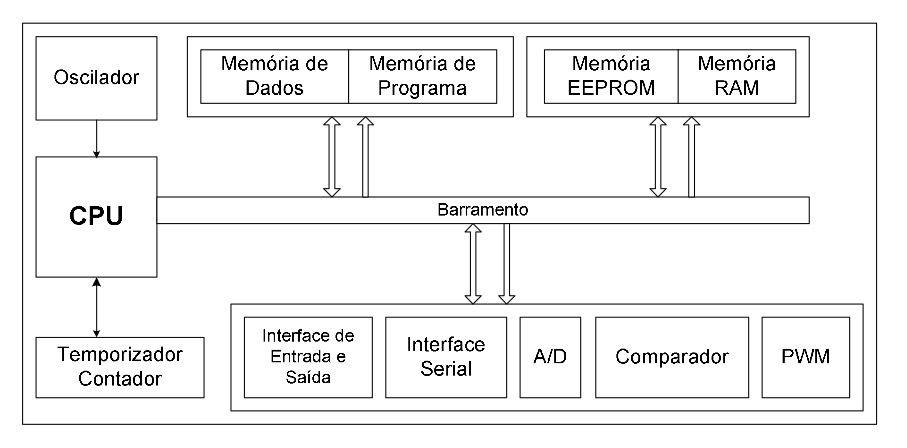
\includegraphics[width=1.0\columnwidth]{images/esquematico_microcontrolador} 
	\caption[Arquitetura de um típico microcontrolador]{Arquitetura de um típico microcontrolador}
	\label{fig:esquematico_microcontrolador} 
	\end{figure}

  Podemos ver na figura \ref{fig:microcontrolador_atmega}, o esquemático de um microcontrolador típico.

  	\begin{figure}[tb]
	\centering 
	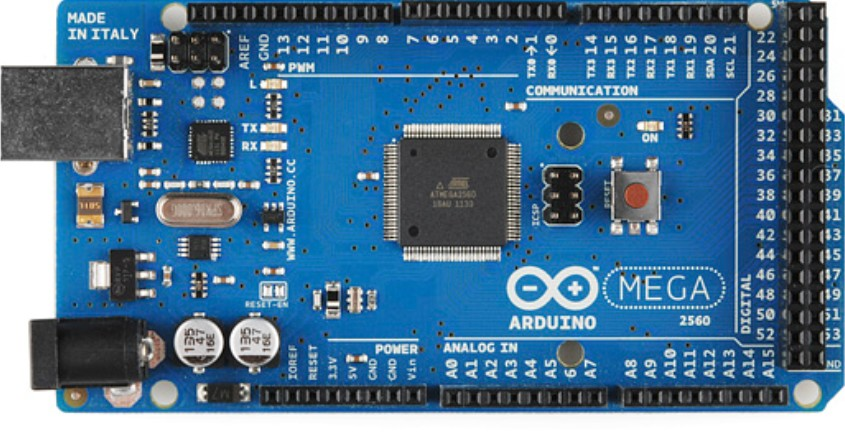
\includegraphics[width=0.5\columnwidth]{images/microcontrolador_atmega} 
	\caption[Microcontralador ATMEGA 2560]{Microcontralador ATMEGA 2560 de 16 MHz utilizado para validação do AG desenvolvido neste trabalho}
	\label{fig:microcontrolador_atmega} 
	\end{figure}

   Neste trabalho, foi dado ênfase ao uso do microcontrolador ATMEGA 2560 que são microcontroladores AVR, da família ATMEL. São microcontroladores, em geral de 8 bits e cuja tecnologia utilizada é o RISC – Reduced Instruction Set Computer e arquitetura harvard. 


  Na arquitetura harvard, há uma separação entre a memória de dados e a memória de programa, por meio de um barramento para cada tipo de memória. Deste modo, há uma redução na quantidade de portas lógicas, o que produz um núcleo de processamento mais compacto e uma programação mais  eficiente (Lima, 2010). Esta arquitetura é mais vantajosa em relação à tradicional arquitetura de Von Neuman que usa um mesmo barramento para ambas as memórias, de dados e do programa. Atualmente há uma tendência para o uso da arquitetura Harvard, que está sendo aperfeiçoada e otimizando cada vez mais  processamento no microcontroladores. É possível alcançar maior economia de energia e execução de mais instruções em poucos ciclos de clock.



  As figuras \ref{fig:arquitetura_von_neuman} e \ref{fig:arquitetura_harvard} mostram o esquemáticos das arquiteturas de Von Neuma e Harvard, respectivamente.

  	\begin{figure}[tb]
	\centering 
	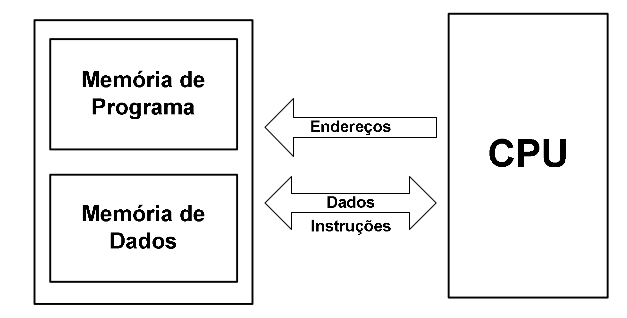
\includegraphics[width=0.5\columnwidth]{images/arquitetura_von_neuman} 
	\caption[Arquitetura Von-Neuman]{Arquitetura Von-Neuman}
	\label{fig:arquitetura_von_neuman} 
	\end{figure}

	\begin{figure}[tb]
	\centering 
	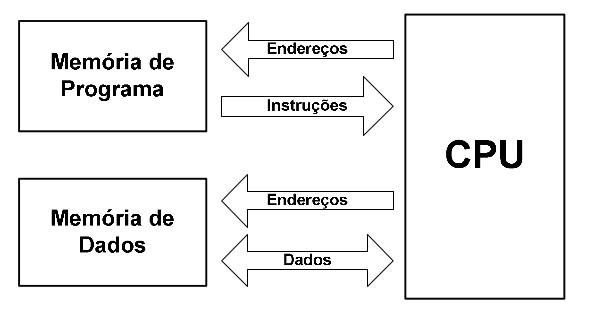
\includegraphics[width=0.5\columnwidth]{images/arquitetura_harvard} 
	\caption[Arquitetura Harvard]{Arquitetura de Harvard}
	\label{fig:arquitetura_harvard} 
	\end{figure}

\chapter{Descrição do projeto}

 Este trabalho tem como finalidade a investigação, otimização e adequação do uso de AGs, em sistemas embarcados, tais como microcontroladores (MuC), microprocessadores (MuP) e sistemas digitais de processamento de sinais (DSPs), frequentemente utilizados em sistemas embarcados para aplicações dedicadas à soluções complexas de engenharia e, deste modo poder ser usado em vários setores da indústria.

 O desenvolvimento deste trabalho esteve concentrado no desenvolvimento de AG em linguagem C, de um modo que pudesse, facilmente, ser adaptado e utilizado em sistemas embarcados diversos.

 O algoritmo foi escrito de modo estruturado com várias funções, permitindo escolher que tipo de procedimento poderá ser usado em cada etapa do GA, podendo, deste modo, avaliar qual método possui melhor desempenho, tanto do ponto de vista da execução em si, quanto dos resultados obtidos para a solução do problema.

 Deste modo foi possível avaliar o tempo de execução do GA com variações na sua execução, como por exemplo, diferentes formas de seleção, podendo esta ser por torneio, roleta simples, roleta de quatro pontos ou a combinação deste métodos. Como o objetivo do trabalho é a investigação do uso de GAs em sistemas embarcados de modo geral, não houve preocupação na solução de um problema específico, mas na otimização geral da execução do algoritmo. Deste modo procurou-se parametrizar todas os aspectos do GA, o máximo que se pode, desde, quantidade de variáveis do problema, até o tamanho do cromossomo, para serem definidas pelo usuário.

\section{Descrição do GA}

 O algoritmo foi divido em várias etapas, sendo elas: iniciação da população, crossover, mutação, e avaliação da população. As três ultimas etapas são repetidas em um laço até que o número de iterações máximo seja atingido ou o critério de busca seja  alcançado.
 No fim de cada iteração a população é avaliada e, para cada cromossomo é calculada uma aptidão, que será utilizada como parâmetro para ordenação da população, que resultará em uma lista, em ordem decrescente de aptidão. A aptidão de cada cromossomo é calculada convertendo os valores de cada cromossomo para a faixa de valores do problema. Em seguida, este valor é avaliado pela função objetivo ou função de avaliação, dando como resultado a aptidão do cromossomo. 

\section{A representação do cromossomo}

  No GA desenvolvido neste projeto, cada cromossomo é representado por um valor inteiro, convencionado no algoritmo como tipo unsigned int. Deste modo a capacidade de representação é limitada pela precisão desejada pelo usuário que pode ser configurada de maneira livre, obedecendo-se as restrições do sistema em que o algoritmo será utilizado.

\section{A precisão do algoritmo}

  A precisão do algoritmo é definida pela quantidade de bits em cada cromossomo. Neste projeto a precisão é um parâmetro global do algoritmo que pode ser configurada pelo usuário de, acordo com a capacidade de representação numérica do sistema que irá executá-lo. Este parâmetro foi definido como constante, não podendo ser mais alterado depois do inicio da execução do algoritmo. Pelos teste realizados, percebeu-se que a precisão escolhida em nada afeta o tempo de execução do algoritmo de modo que a sua escolha é apenas limitada pela capacidade de representação numérica do sistema que irá executar o algoritmo.
  Para sistemas de 10 bits, que á resolução dos conversosres AD/DA da maioria dos microprocessadores, é possível uma representação inteira de até   $2^10 -1$. Isso fornece uma precisão bastante razoável para a solução de problemas de otimização de um modo geral.

\section{Otimização de memória}

  Devido ao propósito do GA ser executado em hardwares de baixa quantidade de memória, comum em sistemas embarcados e por ter sido desenvolvido em linguagem c, fez-se uso extensivo de ponteiros, de modo que grande parte das funções envolvia passagem de parâmetros por referência. Como é o caso da população de cromossomos. Por se tratar de uma matriz de inteiros, esta é alocada em um único espaço de memória, de modo que seu acesso de todo o algoritmo é feito por meio de ponteiros. Nesta matriz, cada linha representa um cromossomo e cada coluna uma variável diferente do problema a ser otimizado.
  A metodologia utilizada levou em conta a avaliação dos tempos de execução de cada etapa do AG para diferentes tamanhos de população e de cromossomos, e a partir daí, procurar otimizar esses tempos a fim de se obter o melhor tempo global de execução.

\section{Inicialização da população}

  A inicialização desta população ocorre a partir da geração de vários cromossomos até preencher toda a população. Cada cromossomo é representado por um número inteiro cujo valor é escolhido randomicamente e cujo valor máximo depende da precisão escolhida para o algoritmo. 

  Neste código, um laço do tipo for é feito, com uma variável de controle do tipo inteiro, cujo valor inicial vai de zero até o tamanho da população menos um. A cada iteração um valor randômico é escolhido conforme a equação  a seguir

  Seja b o valor do cromossomo e p a precisão escolhida , seu valor sorteado será dado pela equação \ref{eq:sorteio_chr}.

  \begin{equation}  
    b = rand() \% MAX\_SORT
    \label{eq:sorteio_chr}
  \end{equation}

  onde rand é uma função da linguagem C que retorna um valor inteiro aleatório, p é a precisão do algoritmo e  MAX\_SORT é definido na equação a seguir 
  \begin{equation}
    MAX\_SORT = 2^p-1
    \label{eq: sort_max}
  \end{equation}

  Além da geração da população inicial há a inicialização de uma variável global chamada sumPopulation que será passada como referência através de um ponteiro para a função de inicialização da população e somará o valor de todos os indivíduos da população. Esta variável será utilizada no método do crossover.

\section{Seleção da nova população}

\subsection{O método da roleta}

  O método de seleção escolhido levou em conta a técnica da roleta de quatro pontos que seleciona quatro indivíduos de uma única vez, que irão cruzar dois a dois e gerar quatro outros novos indivíduos.  Este sorteio consiste em somar todas as aptidões da população e em seguida sortear um número maior que zero e menor do que esta soma. A partir deste sorteio, encontramos o indivíduo cuja aptidão seja a menor possível, mas maior que o valor sorteado.  Com este valor sorteado, encontramos os outros três indivíduos da maneira como é descrita a seguir. 
  Seja  ch1, o cromossomo sorteado no método da roleta simples e N o tamanho da população, os outros três cromossomos, ch2, ch2 e ch3 serão encontrados pelas equações \ref{eq:chr2_roleta}, \ref{eq:chr3_roleta} e \ref{eq:chr4_roleta}.

  \begin{equation}
    ch_2 = (ch1 + dist) \% N
    \label{eq:chr2_roleta}
  \end{equation}
  
  \begin{equation}
    ch_3 = (ch1 + 2*dist)\% N
    \label{eq:chr3_roleta}
  \end{equation}
  
  \begin{equation}
    ch_4 = (ch1 + 3*dist) \% N
    \label{eq:chr4_roleta}
  \end{equation}
 
  onde dist é dado por $dist = \frac{N}{4}$


\subsection{O Crossover}

  O crossover é realizado  “seccionando” os dois cromossomos ao meio e trocando-se a metade menos significativa de um cromossomo pela do outro. Este método é conhecido como crossover de um ponto. Pelo fato dos cromossomos serem representados por valores inteiros, o crossover é realizado por meio de uma operação bit-a-bit, através do qual modificamos a sequência binária de bits que formam cada valor inteiro. Este procedimento tem como efeito reduzir o custo computacional do algoritmo.

  No código a seguir podemos ver como o cruzamento de dois cromossomos ocorre bit a bit.

  \begin{verbatim}
  void cruzaCromossomos(unsigned int* chr1, unsigned int* chr2){
    int chr1_,chr2_;
    int i;
    chr1_ = *chr1;
    chr2_ = *chr2;
    for(i = 0; i < size_chromossome/2; i++){
        if(chr1_ & (1 << i))
            *chr2 |= 1 << i;
        else
            *chr2 &= ~(1 << i);
        if(chr2_ & (1 << i))
            *chr1 |= 1 << i;
        else
            *chr1 &= ~(1 << i);
    }
  }

  \end{verbatim}

\subsection{Mutação}

  No processo de mutação, cada nova geração é avaliada de modo que para cada cromossomo, sorteia-se um valor entre zero e um. Se o valor sorteado for menor ou igual à taxa de mutação, o cromossomo é modificado, trocando um bit em uma posição aleatória na cadeia binária que o representa.
  Um novo valor é sorteado para definir a posição no cromossomo, onde ocorrerá a permutação no bit selecionado. Se o valor do bit for um, será trocado por zero e vice -versa. Esta operação é do tipo binária e ocorre conforme o comando a seguir
  
  \begin{verbatim}
  *ch r ^=  (1 << pos)
  \end{verbatim}

  onde pos é uma variável do tipo inteiro que representa a posição sorteada para a permutação do valor binário.

  O parâmetro desta função é a variável do tipo unsigned int chr, que representa o cromossomo que sofrerá mutação. 

  O sorteio da posição é feito através do comando $pos = rand() \% p$,

  onde p é uma variável global do tipo const int que representa o tamanho cromossomo e que equivale, também, à precisão da busca.

\subsection{Elitismo}
  
  Neste trabalho, a decisão pelo uso do elitismo fica a cargo do usuário, podendo este configurar nas constantes definidas para o AG. para efeito de medição do tempo de execução do algoritmo foi utilizada uma taxa de elitismo de 10\%

\section{Avaliação da população}

  A avaliação da população consiste de três etapas fundamentais. A primeira delas e a normalização dos valores da população para o espaço de busca da solução do problema. Esta normalização é  feita por meio de uma interpolação através da seguinte equação \ref{eq:normalizacao}

  

  Onde mínimo e máximo são os limites do espaço de busca do domínio da função de avaliação que se quer minimizar. 

  Logo que a população é normalizada, é calculada sua aptidão por meio da função de avaliação.

  Existem dois vetores que representam a população. Um contem os valores dos cromossomos, do tipo inteiro e outro do tipo float, que guarda o valor da aptidão do cromossomo do índice correspondente. 

  Após o cálculo da aptidão, a população é ordenada em ordem decrescente, de modo que o cromossomo mais apto, que é o de menor valor, ficará no topo do vetor de ordenação e o menos apto, ficará no fim do vetor. A ordenação toma como referência a aptidão da população, mas esta ordenação ordenação ocorre também sobre o vetor da população em si, com os valores inteiros. Para este procedimento foi utilizado o já conhecido algoritmo quicksort.

\section{Normalização da população}

  A normalização dos cromossomos ocorre na etapa de avaliação da população e tem como objetivo converter os valores dos cromossomos do tipo inteiro para o range do problema de otimização, para em seguida calcular a aptidão de cada cromossomo.

  Um laço do tipo for percorre o vetor com a população de indivíduos e em cada iteração uma função  de normalização é chamada, passando como parâmetro o valor do cromossomo a ser normalizado, os valores mínimo e máximo do intervalo da busca e o valor máximo da população.
  
  Na função de normalização finalidade de converter o valor de cada indivíduo da população para seu valor correspondente dentro do intervalo de valores de busca definido para o problema.  Os valores dos indivíduos da população estão no formato inteiro e podem ser bastante elevados, de modo a ficarem fora do range da busca do problema.

 A normalização  de cada indivíduos é feita  através da equação 
 

 onde as variáveis mínimo e máximo são os valores limites do intervalo da busca; MAX\_SORT é o maior valor dentre os indivíduos da população e chr é o valor do cromossomo que se quer normalizar.

\section{A aptidão dos cromossomos}

  Como este trabalho não deteve-se em otimizar um problema específico, mas investigar o desempenho do uso de GA em sistemas embarcados, a função de avaliação utilizada foi a mais simples possível, de modo que sua execução interferisse o mínimo possível na avaliação do tempo de execução do AG.

  Esta função é usada para calcular o valor de aptidão da população. Um laço percorre o vetor da população e em cada iteração, o valor do cromossomo na forma normalizada é passado como parâmetro na chamada da função de avaliação que irá retornar o valor da aptidão do cromossomo.

  A função de avaliação usada neste trabalho, para fins apenas de teste foi definida como $f(x) = x$.

\section{Valores randômicos}

  Os AGs, de um modo geral são bastante dependentes da valores gerados de modo pseudoaleatórios, pois são estes valores que dão ao algoritmo sua natureza estocástica, a fim de que seu comportamento se aproxime o máximo possível do aspecto evolutivo biológico, observado na natureza. No entanto, o microcontrolador utilizado neste trabalho não possui a biblioteca time.h, normalmente utilizada para criação da semente na chamada da função srand, que é responsável pela geração de valores aleatórios em linguagem C. Por este motivo, a semente usada no algoritmo foi pega do contador TCTNT1  que é incrementado via clock interno. 
  TCCRA/B -  Timer/Counter Control Register

\section{Configuração do Registrador de controle TCCR1B}

  O registrador possui 8 bits, os quais foram configurados da seguinte maneira:\\
  \textbf{BIT 7 – ICNC1:}  input Capture Noise Canceler. Este bit foi colocado em 0, pois o pino de captura ICP1 não é necessário.\\
  \textbf{BIT 6 – ICES1:} Input Capture Edge Select. Este bit foi colocado em 0 também, pois define em qual borda, se de subida ou decida, o valor do contador será copiado para o registrador ICR1. Logo, é indiferente, qual borda isso ocorre, para os fins deste contador.\\
  \textbf{BIT 4,3 – WGM13:2:} Waveform Edge Generation Mode. É responsável pela forma da onda será empregada na contagem do contador. Foi deixado em 0, gerando uma onda normal, com atualização imediata.\\
  \textbf{BIT 2:0 – CS12:0:} Click Select. Este três últimos bits são responsáveis pela escolha do clock. São rotulados como CS12, CS11, CS10 e sua configuração foi definida como CS12 = 0, CS11 = 0, CS10 = 1, que significa que não há divisão do clock. \\


  Deste modo a configuração do registrador TCCR1B fica definida como 

  \begin{verbatim}
    TCCR1B |= 0b00000001;
  \end{verbatim}

\section{A validação do algoritmo}

  A validação do algoritmo foi feita através do microcontrolador ATMEGA  Numero do atmega
  A validação do AG foi feita, medindo-se os tempos de execução de cada etapa do AG através de um osciloscópio de bancada. A medição do tempo foi feita de modo indireto, usando-se a frequência gerada por um sinal de saída no pino digital 13  do ATMEGA. O A saída desta porta alterna entre nível baixo e nível alto a cada iteração do laço de execução do AG. O sinal desta porta é capturado pelas pontas de prova do osciloscópio que exibe na tela do computador uma onda quadrada através da qual podemos medir sua frequência. Esta frequencia é o tempo gasto para a execução do algoritmo dentro do laço, conforme o trecho de código a seguir.

  \begin{verbatim}
  while(1){  
        seed = TCNT1;
        srand(seed);        
        if (t % 2 == 0)
            PORTB |= 0b10000000;
        else
            PORTB &= 0b01111111; 
        t++;        
        getNewPopulation(population, newPopulation,aptidao);
        getAptidao(aptidao,newPopulation);        
        avaliaPopulacao(newPopulation,aptidao);       
        transferePopulacao(population,newPopulation,size_population);                 
  }
  \end{verbatim}

\section{Resultados}
	
  Os resultados obtidos podem ser observados pelas imagens a seguir. Diversas medições foram realizadas a fim de se observar o tempo de execução do AG para cada configuração diferente.

  Teste foram realizados para medir o desempenho do AG, variando-se o tamanho de sua população e deixando-se fixo a precisão desejada. Esta configuração propõe otimizar uma função de uma única variável, cuja função objetivo é $f(x) = x$  Os resultados são mostrados no gráfico da figura \ref{fig:populacao_tempo}.

    \begin{figure}[tb]
	\centering 
	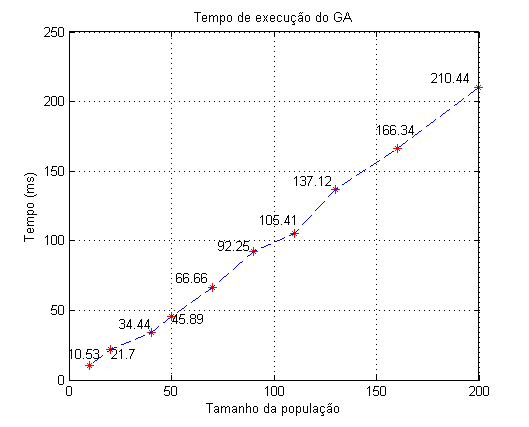
\includegraphics[width=1.0\columnwidth]{images/1_var_prec_10_sizepop_x_t} 
	\caption[Tempo de execução x Tamanho da população]{Tempo de execução x tamanho da população}
	\label{fig:populacao_tempo} 
	\end{figure}

  Os teste também foram realizados para o caso de uma população de tamanho fixo em 80 cromossomos e precisão de 10 bits, porém variando-se a quantidade de variáveis na função objetivo. Os resultados obtidos são mostrados no gráfico da figura \ref{fig:qtdvar_tempo}.

  	\begin{figure}[tb]
	\centering 
	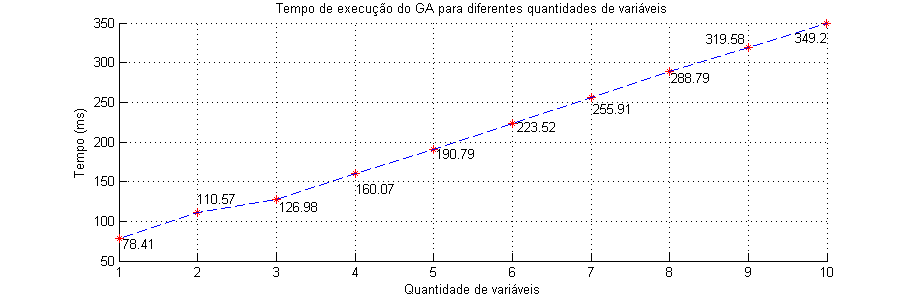
\includegraphics[width=1.0\columnwidth]{images/N_variaveis} 
	\caption[Tempo de execução x Quantidade de variáveis]{Tempo de execução x Quantidade de variáveis}
	\label{fig:qtdvar_tempo} 
	\end{figure}

  Além dos tempos de execução em relação ao tamanho da população e da quantidade de variáveis, também foi investigada a influência da variação na precisão do algoritmo, tomando-se como base uma população de 70 indivíduos e considerando apenas uma variável. Os resultados obtidos são mostrados no gráfico da figura \ref{fig:tempo_precisao}.

  	\begin{figure}[tb]
	\centering 
	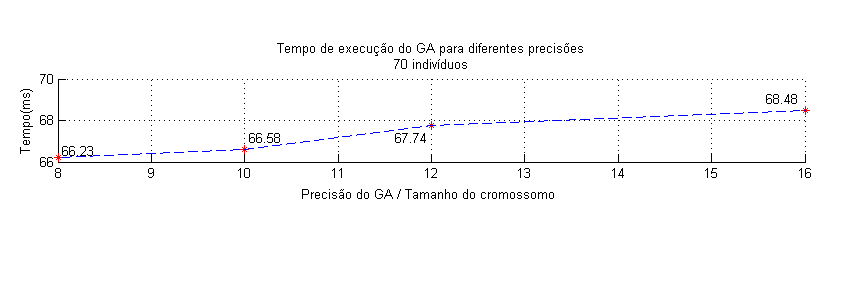
\includegraphics[width=1.0\columnwidth]{images/precisao_x_tempo} 
	\caption[Tempo de execução x Precisão]{Tempo de execução x Precisão}
	\label{fig:tempo_precisao} 
	\end{figure}

  A partir destas medições, percebe-se que a precisão dobrou, enquanto o tempo de execução aumentou cerca de duas unidades, o que mostra que a precisão deseja para o AG é uma limitação mais do microcontrolador do que do algoritmo em si. Para microcontroladores mais robustos é possível optar por uma maior precisão sem que isso aumente o tempo de execução do AG.

  Medições foram realizadas a fim de avaliar quanto tempo é gasto na execução de cada etapa do AG. Pelo fato do AG ser  dividido em várias etapas, decidiu-se avaliar o tempo de execução dos principais procedimentos do algoritmo. São eles: Seleção da nova população, cálculo de aptidão e avaliação da população. A seleção da nova população possui como principais métodos, o crossover e a mutação, etapas bastante característica de uma AG, por isso seus tempos individuais de execução foram avaliados.

  Para um AG de 100 indivíduos, com precisão de 10 bits e uma variável, obteve-se os seguintes tempos.

 Tempo total daexecução do AG:  105.66 ms
 seleção da nova população: 67.64 ms
	crossover: 45.64 ms
	mutação 67.64 ms
 Cálculo da aptidão: 23.18 ms
 Avaliação da população: 12.09 ms

 Estes são os principais procedimentos do AG desenvolvido neste projeto. O tempo de outros procedimentos auxiliares do algoritmo não foi medido. Por esta razão a soma dos tempos individuais não dá exatamente o tempo total da execução do algoritmo. Esta tempos “faltantes” se devem a estes trechos de códigos auxiliares.




% ----------------------------------------------------------
% Capitulo com exemplos de comandos inseridos de arquivo externo 
% ----------------------------------------------------------

\include{abntex2-modelo-include-comandos}

% ---
% Finaliza a parte no bookmark do PDF
% para que se inicie o bookmark na raiz
% e adiciona espaço de parte no Sumário
% ---
\phantompart
% ---
% Conclusão
% ---

\chapter[Conclusão]{Conclusão}

  Este trabalho consistiu na implementação de um AG em linguagem C, com o objetivo de investigar o desempenho destes algoritmos em sistemas embarcados baseados em microcontroladores. Os tempos de execução obtidos a partir dos testes realizados, mostra que é viável o uso de AGs em sistemas embarcados com o objetivo de solucionar problemas complexos, de várias variáveis, como também criar sistemas de baixo consumo e pequeno porte, devido, também, à própria arquitetura dos microcontroladores que estão cada vez mais otimizados. Os testes realizados consideraram diferentes configurações de parâmetros como tamanho da população, precisões variadas e diferentes quantidades de variáveis, podendo  atender diversos tipos de aplicações. Os tempos obtidos são bastante razoáveis, como observado nos dados, observou-se um tempo de 45.89 ms para uma população de 50 indivíduos. Esse tamanho de população é razoável para a solução de um problema de otimização. Com relação à precisão do AG, observou-se que o tamanho do cromossomo não influencia tanto no desempenho do do algoritmo. Para uma variação de 8 bits para 16 bits, observou-se uma variação de apenas cerca de 2 ms. A  grande maioria dos microcontroladores possuem conversores AD/DA de até 10 bits de precisão e que populações de cinquenta indivíduos são bem razoáveis pra a solução de um problema de otimização. Isso mostra que para estas aplicações, o tempo de resposta será bastante aceitável

\chapter[Perspectivas futuras]{Perspectivas futuras}

  fA partir dos resultados obtidos neste projeto, conclui-se que o uso de GAs em sistemas embarcados é viável, apesar dos recursos limitados de memória e processamento, pois apresentam tempos de resposta satisfatórios. As perspectivas futuras são as de que melhores resultados podem ser alcançadas distribuindo-se a execução do algoritmo em vários microcontroladores, por meio de interfaces de comunicação simples como I2C, através de da criação de um protocolo de dados a fim de se obter tempos melhores. Além disso,  é desejável que o algoritmo possa ser testado em outros plataformas, como microcontroladores da família PIC, Raspberry PI, BeagleBone, entre outros. 

%\lipsum[31-33]

% ----------------------------------------------------------
% ELEMENTOS PÓS-TEXTUAIS
% ----------------------------------------------------------
%\postextual

% ----------------------------------------------------------
% Referências bibliográficas
% ----------------------------------------------------------

%Lima \cite{souza} has proposed that...

% http://www.apogeeu.fee.unicamp.br/sites/apogeeu.fee.unicamp.br/files/Aula2.pdf

\addcontentsline{toc}{section}{Referências}
\begin{thebibliography}{99}

\bibitem{souza} DE SOUZA, ALISSON ; FERNANDES, MARCELO . Parallel Fixed Point Implementation of a Radial Basis Function Network in an FPGA. Sensors (Basel), v18223­18243,2014.
\bibitem{marcelo} DE SOUZA, ALISSON C. D. ; FERNANDES, MARCELO A. C. . Proposal for parallel fixed point implementation of a radial basis function network in an FPG IX Southern Conference on Programmable Logic (SPL), 2014, Buenos Aires. 2014 IX Southern Conference on Programmable Logic (SPL), 2014. 
\bibitem{dhanajay} Dhananjay Gadre. Programming and Customizing the AVR Microcontroller. McGraw­Hill. 2002.]
[4] Joe Pardu. C Programming for Microcontrollers Featuring ATMEL's AVR Butterfly and the free WinAVR Compiler. Smiley Micros. 2005.
\bibitem{richard}  Richard H. Barnett, Sarah Cox, Larry O'Cull. Embedded C Programming and the Atmel AVR. Thomson Delmar Learning; 2 edition. 2006.
\bibitem{simon}  Simon Haykin. Neural Networks: A Comprehensive Foundation (3rd Edition). Prentice­Hall, Inc., Upper Saddle River, NJ, USA, 2007.
\bibitem{rosa} ROSA, João Luís Garcia. Fundamentos da inteligência artificial. Rio de Janeiro: LTC, 2011. 212 p.ISBN: 9788421605935. 
\bibitem{coppin}  COPPIN, Ben; VALÉRIO, Jorge Duarte Pires. Inteligência artificial. Rio de Janeiro: LTC, 2010. 636 p. ISBN: 9788521617297.
\bibitem{Lima} LIMA, Charles Borges de. AVR e Arduino : técnicas de projeto / Charles Borges de Lima, Marco Valério Miorim Villaça. 2. ed. – Florianópolis: Ed. dos autores,2012. 632 p.: il; 21,0 cm. ISBN: 978-85-911400-1-5
\end{thebibliography}




% ----------------------------------------------------------
% Glossário
% ----------------------------------------------------------
%
% Consulte o manual da classe abntex2 para orientações sobre o glossário.
%
%\glossary

% ----------------------------------------------------------
% Apêndices
% ----------------------------------------------------------

% ---
% Inicia os apêndices
% ---
\begin{apendicesenv}

% ----------------------------------------------------------
\chapter{}
% ----------------------------------------------------------

\lipsum[50]

% ----------------------------------------------------------
\chapter{}
% ----------------------------------------------------------
\lipsum[55-57]

\end{apendicesenv}
% ---


% ----------------------------------------------------------
% Anexos
% ----------------------------------------------------------

% ---
% Inicia os anexos
% ---
\begin{anexosenv}


% ---
\chapter{}

\chapter{}

\chapter{}
% ---

\lipsum[32]

\end{anexosenv}

%---------------------------------------------------------------------
% INDICE REMISSIVO
%---------------------------------------------------------------------

\phantompart

\printindex


\end{document}

\grid
